%% 
%% Copyright 2007-2025 Elsevier Ltd
%% 
%% This file is part of the 'Elsarticle Bundle'.
%% ---------------------------------------------
%% 
%% It may be distributed under the conditions of the LaTeX Project Public
%% License, either version 1.3 of this license or (at your option) any
%% later version.  The latest version of this license is in
%%    http://www.latex-project.org/lppl.txt
%% and version 1.3 or later is part of all distributions of LaTeX
%% version 1999/12/01 or later.
%% 
%% The list of all files belonging to the 'Elsarticle Bundle' is
%% given in the file `manifest.txt'.
%% 
%% Template article for Elsevier's document class `elsarticle'
%% with harvard style bibliographic references

\documentclass[12pt]{elsarticle}

%% Use the option review to obtain double line spacing
%% \documentclass[authoryear,preprint,review,12pt]{elsarticle}

%% Use the options 1p,twocolumn; 3p; 3p,twocolumn; 5p; or 5p,twocolumn
%% for a journal layout:
%% \documentclass[final,1p,times,authoryear]{elsarticle}
%% \documentclass[final,1p,times,twocolumn,authoryear]{elsarticle}
%% \documentclass[final,3p,times,authoryear]{elsarticle}
%% \documentclass[final,3p,times,twocolumn,authoryear]{elsarticle}
%% \documentclass[final,5p,times,authoryear]{elsarticle}
%% \documentclass[final,5p,times,twocolumn,authoryear]{elsarticle}

%% For including figures, graphicx.sty has been loaded in
%% elsarticle.cls. If you prefer to use the old commands
%% please give \usepackage{epsfig}

%% The amssymb package provides various useful mathematical symbols
\usepackage{amssymb}
%% The amsmath package provides various useful equation environments.
\usepackage{amsmath}
%% The amsthm package provides extended theorem environments
%% \usepackage{amsthm}
\usepackage[colorinlistoftodos,textsize=footnotesize]{todonotes}
%% The lineno packages adds line numbers. Start line numbering with
%% \begin{linenumbers}, end it with \end{linenumbers}. Or switch it on
%% for the whole article with \linenumbers.
%% \usepackage{lineno}
\usepackage{cleveref}
\usepackage{tabularx}


\journal{Acta Astronautica}

\begin{document}

\begin{frontmatter}

%% Title, authors and addresses

%% use the tnoteref command within \title for footnotes;
%% use the tnotetext command for theassociated footnote;
%% use the fnref command within \author or \affiliation for footnotes;
%% use the fntext command for theassociated footnote;
%% use the corref command within \author for corresponding author footnotes;
%% use the cortext command for theassociated footnote;
%% use the ead command for the email address,
%% and the form \ead[url] for the home page:
%% \title{Title\tnoteref{label1}}
%% \tnotetext[label1]{}
%% \author{Name\corref{cor1}\fnref{label2}}
%% \ead{email address}
%% \ead[url]{home page}
%% \fntext[label2]{}
%% \cortext[cor1]{}
%% \affiliation{organization={},
%%            addressline={}, 
%%            city={},
%%            postcode={}, 
%%            state={},
%%            country={}}
%% \fntext[label3]{}

\title{A Spectral Signature-Based Framework for Satellite Reconstruction Using Deep Learning} %% Article title

\author[1]{Yaorong Xiao}
\author[2]{Noah Lewis}
\author[3]{Elena Plis}
\author[3]{Douglas Hope} 
\author[4]{Fabien Baron} 
\author[4]{Stuart M. Jefferies} 
\author[1]{Sergey Plis} 

%% Author affiliation
\affiliation[1]{TReNDS Center & Georgia State University ,%Department and Organization
            addressline={55 Park Pl NE}, 
            city={Atlanta},
            postcode={30303}, 
            state={GA},
            country={USA}}



\affiliation[2]{{National Research Council Post-Doctoral Fellowship Program},%Department and Organization
            addressline={500 5th St NW}, 
            city={Washington},
            postcode={20001}, 
            state={DC},
            country={USA}}
            
\affiliation[3]{organization={Electro-Optical Systems Laboratory (EOSL), Georgia Tech Research Institute (GTRI)},%Department and Organization
            addressline={925 Dalney St}, 
            city={Atlanta},
            postcode={30318}, 
            state={GA},
            country={USA}}


\affiliation[4]{organization={Department of Physics and Astronomy, Georgia State University},%Department and Organization
            addressline={25 Park Place}, 
            city={Atlanta},
            postcode={30303}, 
            state={GA},
            country={USA}}

%% Abstract
\begin{abstract}
%% Text of abstract
Identifying and monitoring residential satellites in Earth's orbit is a difficult task due to vast distances, low sensor resolution, complex tracking, and variable lighting. Moreover, the space environment is harsh, leading to spacecraft degradation from many different sources, including high-energy electrons. These charged particles can induce material degradation, disrupt onboard systems, and reduce the operational lifespan of satellites, thereby complicating both detection and long-term monitoring efforts. To address these challenges, this paper introduces a deep learning approach for reconstructing satellite shape and determining material composition from ground-based hyperspectral images. The method's core innovation is a synthetic data generation technique that creates an unlimited, diverse training set of varying shapes, orientations, and material combinations, all grounded in real-world spectral measurements. This is supported by a comprehensive spectral library of materials including metals, polymers, and solar components, in both pristine and exposed to space-simulated environment  states, to ensure physical realism and simulate varied observation conditions. The resulting models, trained using this system and a supervised learning approach, are separately demonstrated to effectively predict both the satellite's material composition and its shape.

\end{abstract}

%%Graphical abstract
%\begin{graphicalabstract}
%\centering{}
%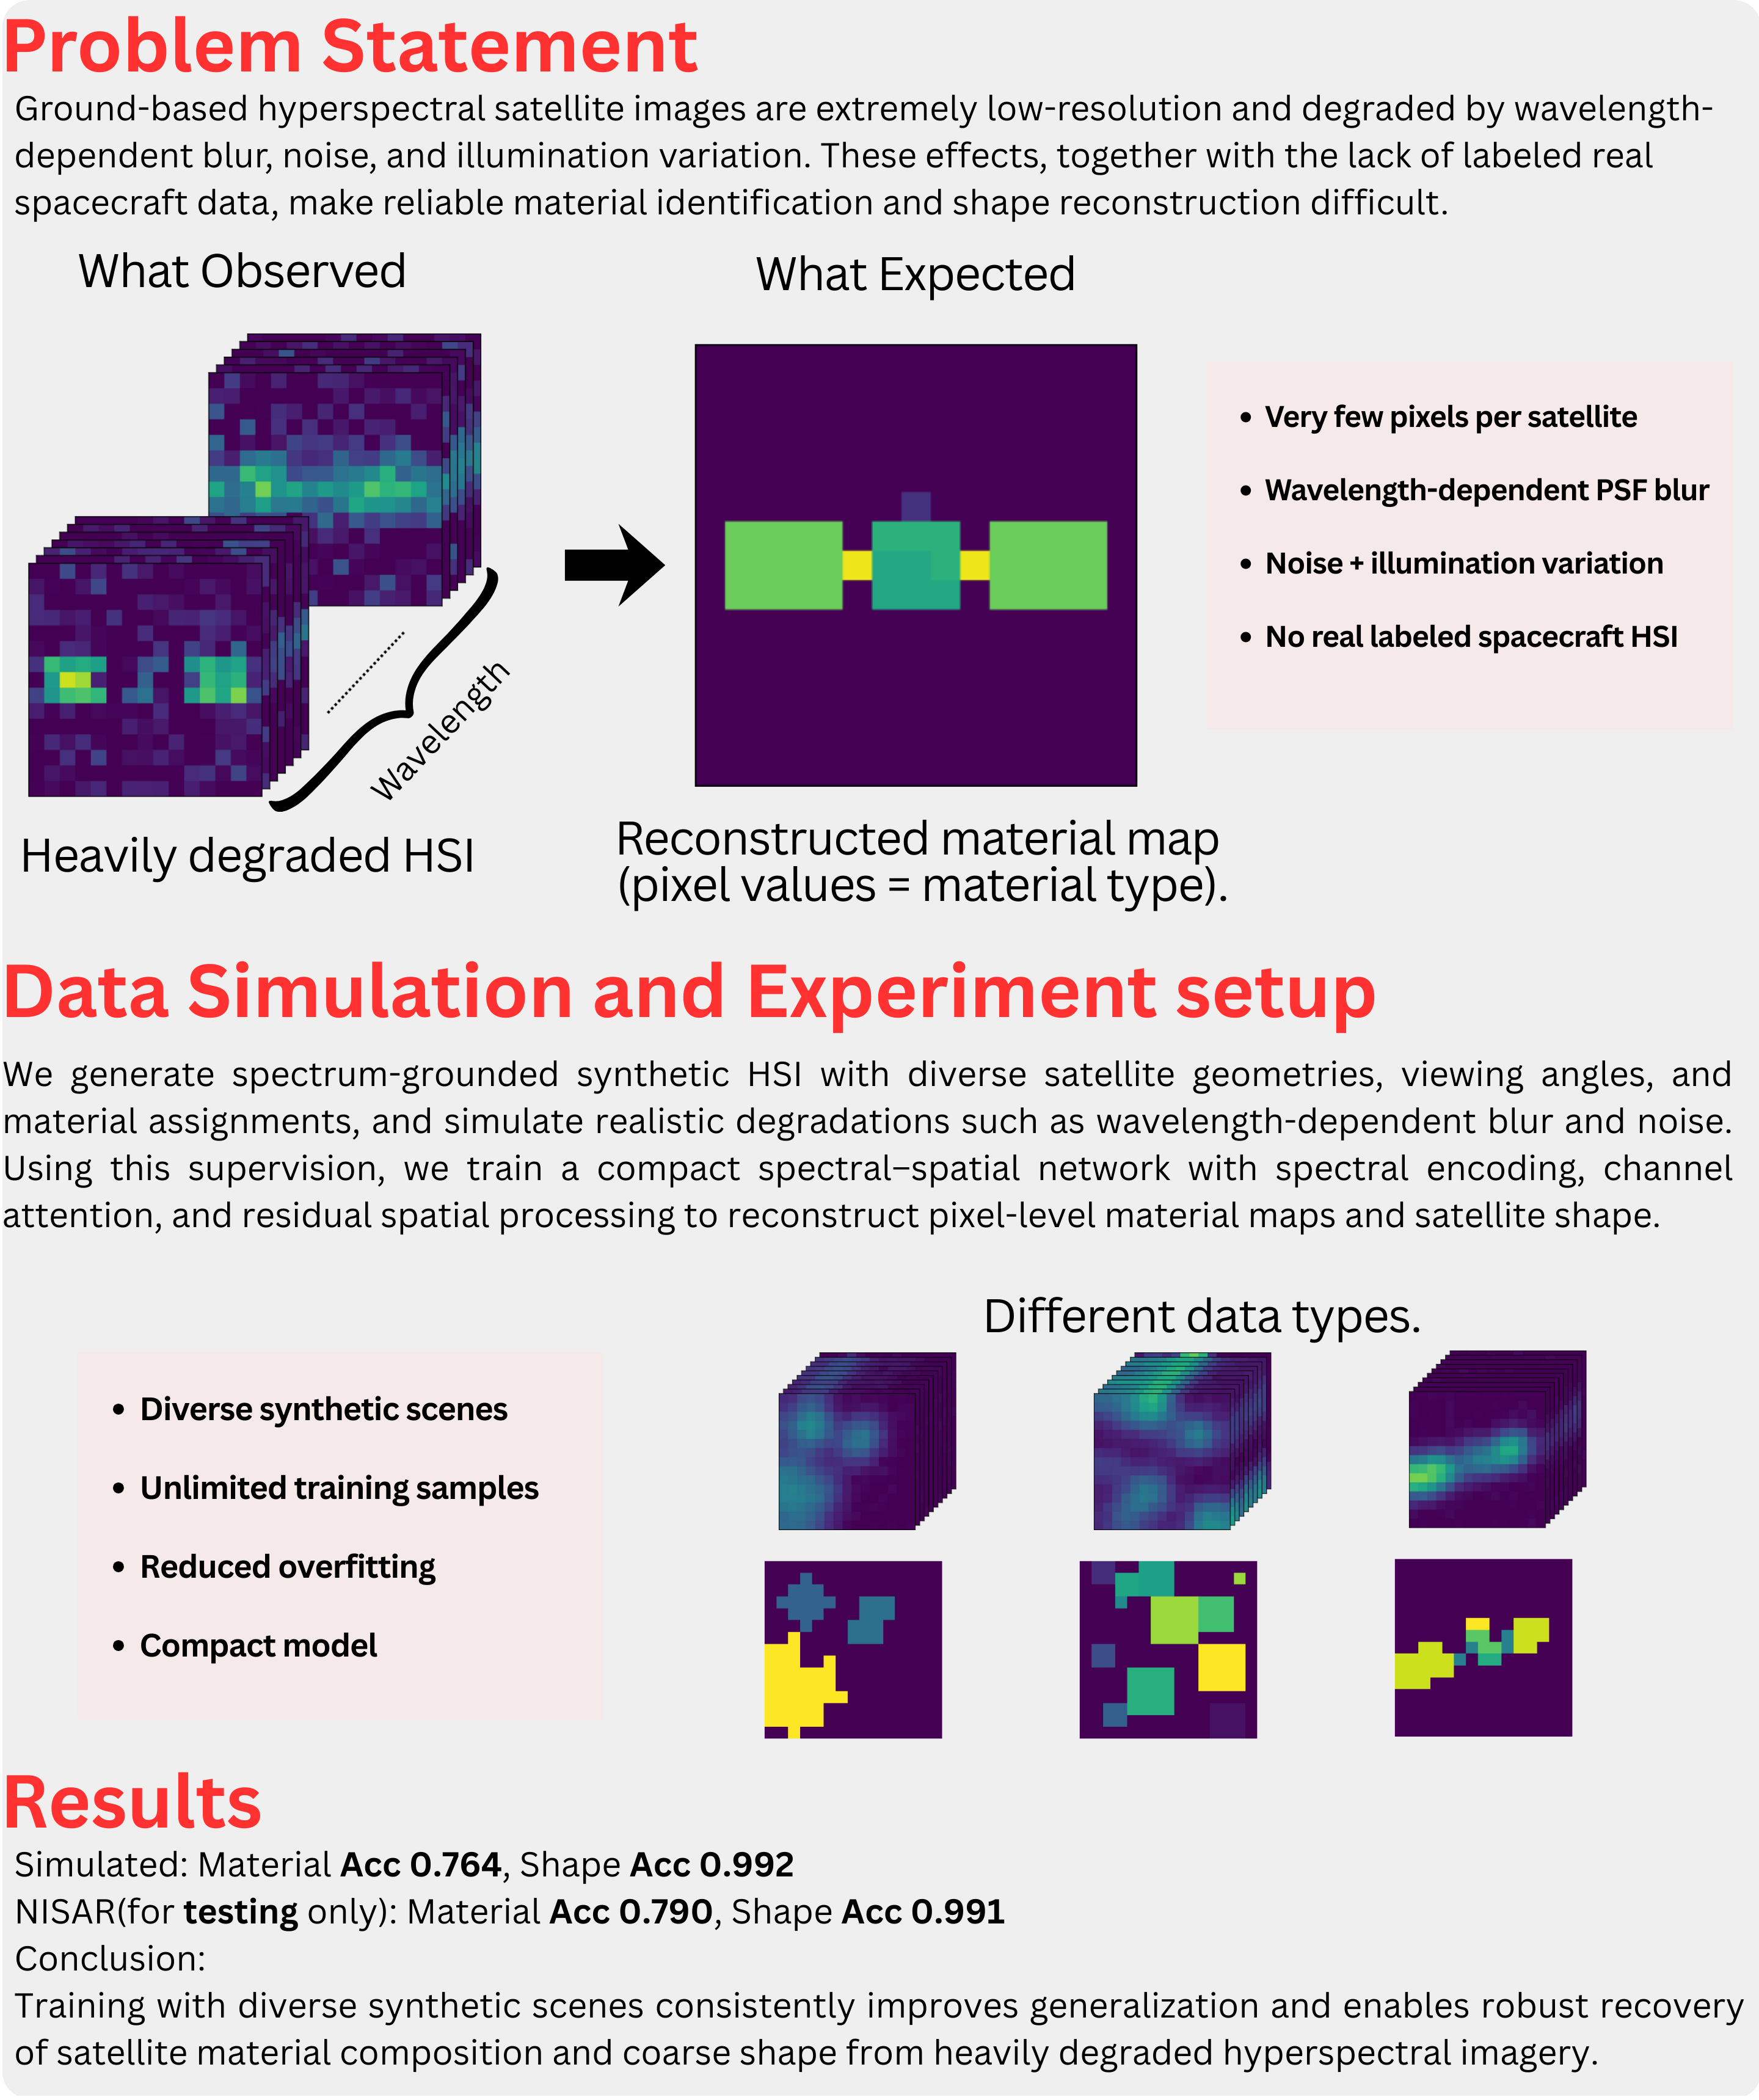
\includegraphics[width=0.97\textwidth]{pdfs/graphical_abstract.png}
%\end{graphicalabstract}

%%Research highlights
\begin{highlights}
\item Spectrum-grounded synthetic pipeline for hyperspectral SSA.
\item Spectral–spatial network for pixel-level material and shape recovery.
\item Dynamic scene mixing improves generalization to unseen structures.
\item Accurate material and shape recovery from low-resolution HSI.
\end{highlights}

%% Keywords
\begin{keyword}
Hyperspectral Imaging
\sep Deep Learning
\sep Satellite Identification
\sep Synthetic Data Generation
\sep Material Composition

\end{keyword}
%% keywords here, in the form: keyword \sep keyword

%% PACS codes here, in the form: \PACS code \sep code

%% MSC codes here, in the form: \MSC code \sep code
%% or \MSC[2008] code \sep code (2000 is the default)

\end{frontmatter}

%% Add \usepackage{lineno} before \begin{document} and uncomment 
%% following line to enable line numbers
%% \linenumbers

%% main text
%%

%% Use \section commands to start a section
\section{Introduction}
Space, across low-Earth (LEO) and Geostationary (GEO) orbit, constitutes strategically vital real estate, hosting a wide array of satellites that support critical functions such as telecommunications, meteorological observation, and broadcast services. Satellites in LEO are vital for communications and defense, where the regime is crowded and comparatively accessible. Due to the crowded nature of LEO, and the speed with which these satellites travel (upwards of one Earth orbit every 90 minutes), these factors culminate in additional tracking and identification difficulties.

LEO contains many vital resources, including the International Space Station (ISS) and the Hubble telescope. This requires finely-tuned and capable defense, which relies on identifying and tracking possible threats to these resources. If an unidentified asset was to pose a threat to these resources, the results could be catastrophic. This is where advanced identification methods are required.

Conversely, a key advantage of GEO is its unique characteristic of maintaining a fixed position relative to specific points on Earth's surface. This geostationary positioning enables continuous coverage of designated terrestrial regions. Additionally, GEO satellites provide extensive coverage due to their high-altitude vantage point; with careful placement, a relatively small constellation can deliver near-global service, extending connectivity to remote and under-served areas worldwide. These advantageous properties of GEO have contributed to the growing congestion within the GEO belt. Identifying and characterizing satellites in GEO remains a significant and growing space situational awareness (SSA) challenge~\cite{xu2019algorithms, siddique2024detection}.  However, the task is complicated by a range of environmental and observational constraints inherent to these orbital regimes.

Unlike LEO, where satellites are relatively close to Earth, enabling high-resolution surveillance and frequent overpasses, GEO  presents the dual difficulties of vast distances and slower relative motions~\cite{sukhov2015some}. These factors result in diminished sensor resolution and weaker signal returns, hindering the ability to discern fine structural details such as solar panel configuration or surface degradation. The remote nature of these orbits also means that objects may remain in the same position relative to an Earth-based observer or may move slowly across the sky, requiring prolonged observation times to collect meaningful data on orbital behavior and object attributes.

Compounding these challenges are variable lighting conditions that can affect the visibility and reflectivity of satellite surfaces. Phenomena such as low phase angles, backlighting during twilight hours, or insufficient solar illumination during certain orbital segments can dramatically reduce the efficacy of optical sensing systems~\cite{campbell2024stingray}. These conditions not only obscure surface features but may also complicate efforts to derive material properties or detect anomalous behavior.

To overcome these difficulties in both LEO and GEO, advanced sensing modalities, including multi-spectral or hyperspectral imaging~\cite{zhao2016multicolor, vasile2024space}, radar~\cite{guarnieri2015advanced, benson2021radar}, and space-based sensors~\cite{scott2016combined}, must be employed alongside sophisticated data processing algorithms~\cite{scorsoglio2024orbit} and predictive modeling techniques~\cite{lee2025application}. Furthermore, accurate identification often depends on detailed prior knowledge of satellite construction materials, design specifications, and operational characteristics~\cite{richmond2017satellite, krag2024innovative}. 

In this work, we present an approach for deep learning reconstruction of satellite shape and detect their 
material composition from ground-based hyperspectral images. The core of the approach is synthetic data 
generation that provides an unlimited data stream of varying shapes, orientation, distortions, and material 
variations, while fundamentally grounded in real-world spectral measurements. These measurements 
serve as the empirical basis for generating synthetic training data, enabling accurate material classification 
from space-based observations. Synthesized distortions simulate wide variance of conditions that are 
impossible to measure in the real-world, while keeping the ground truth for model training.

\section{Synthetic Data Generation}

Images of GEO objects captured by ground-based telescopes can vary substantially. 
Because there is little prior knowledge about what types of objects may appear in space, simulations based on specific object models are unlikely to be representative enough for training a robust model. 
Even when considering satellites alone, their shapes and sizes differ widely depending on their functions, and these differences become even more difficult to distinguish in very low-resolution images. 
However, although the detailed physical properties of the objects are unknown, the image formation process and the main factors that degrade image quality (e.g., optical blur, atmospheric turbulence, and sensor noise) are relatively well understood. 
This makes it possible to simulate the imaging process using a simplified model rather than collected by highly advanced telescope. Under this assumption, large-scale synthetic datasets can be generated, enabling the use of supervised deep learning strategies for training.

To more rigorously evaluate the model training process, we generated a synthetic dataset used for training our model to predict existing materials. This data synthesis process consists of three major stages: (1) spectral library preparation, (2) scene and label generation, and (3) HSI generation. These steps ensure that both the spectral properties of real aerospace materials and the wavelength-dependent imaging degradations observed in practice are reflected in the data.

%Furthermore, we plan to simulate objects with as much shape diversity as possible to help the model learn material properties from highly degraded hyperspectral images (HSIs). Such a strategy is expected to be particularly effective for learning from overlapped or mixed spectral signatures originating from multiple materials within a single pixel. By constructing a large-scale synthetic database with rich and diverse feature variations, we get an opportunity to approximate real GEO observations and thereby improve the model’s robustness and generalization ability.

\subsection{Spectral library preparation}

\begin{figure}
    \centering
    \includegraphics[width=0.8\linewidth]{pdfs/material_generation.pdf}
    \caption{Synthetic spectrum generation pipeline (material: Elgiloy). \textbf{(a)} Absolute reflectance spectra for the pristine and irradiated material conditions. \textbf{(b)} Generation of an intermediate spectrum by linear interpolation between the pristine and irradiated spectra using a randomly sampled mixing coefficient $w \in [0,1]$. \textbf{(c)} Simulation of atmospheric disturbances by adding zero-mean Gaussian noise to the interpolated spectrum, producing the final synthetic material observation.}
    \label{material_generation}
\end{figure}

The simulation begins with a list of measured directed hemispheric reflectance (DHR) representing materials commonly used in spacecraft structures, including metals, polymers, solar array cover glasses, solar cell coupons, ad paints. The dataset incorporates materials collected from multiple sources, including research campaigns focused on exposing various materials to a space-simulated environment, particularly high-energy electron irradiation, which is the dominant component of the GEO environment, previously conducted by~\cite{plis2021effect,reyes2021spectroscopic, plis2022characterization, plis2023ground}, as well as publicly available data from open literature~\cite{reyes2023analysis,reyes2018characterization, jorgensen2001spectral}, and the NASA Spectral Library. 


All reflectance spectra are first resampled onto a common wavelength grid uniformly spanning 350–1000 nm. 
To align material wavelength obtained from different sources,
we apply linear interpolation across wavelength so that each spectrum is matched at the same set of wavelength points, even when the original measurements were collected at slightly different wavelengths. This resampling step provides consistent spectral dimensionality across all materials and prevents artifacts that could arise from uneven wavelength spacing in downstream processing.

To model realistic material degradation patterns, we also account for radiative exposure experienced by spacecraft materials in orbit. In this case, the pristine and irradiated spectra of each material are combined using a linear interpolation between the two exposure conditions, allowing each simulated spectrum to transition smoothly between pristine and irradiated state: 
\[
\mathbf{s} \;=\; \mathbf{s}_{\text{pris}} 
\;+\; w\,\big(\mathbf{s}_{\text{irr}} - \mathbf{s}_{\text{pris}}\big),
\qquad w \in [0,1].
\]
This convex combination captures gradual degradation behavior and represents the range of exposure levels encountered in operational space environments. 

To simulate the spectral imperfections introduced by atmospheric scattering, sensor noise, and illumination imbalance in real orbital hyperspectral measurements, we introduce a small Gaussian perturbation to every material’s simulated reflectance. These effects ensure that the observed spectrum does not appear as a perfectly smooth curve, regardless of whether the surface has experienced radiation exposure.
The complete mixing model is expressed as:
\begin{equation}
\mathbf{s}_m 
= (1-w)\,\mathbf{s}_{pris}
+ w\,\mathbf{s}_{irr}
+ \epsilon,
\qquad w \in [0,1],
\end{equation}
where \(\epsilon \sim \mathcal{N}\!\bigl(0,\,\sigma_m^2\bigr)\) 
represents atmospheric and sensor induced spectral variation added to that material’s reflectance. The noise scale \(\sigma_m\) is set as a small fraction of the material’s intrinsic variability, for example 
\(\sigma_m = \alpha\cdot\mathrm{std}(\mathbf{s})\) with 
\(\alpha \in (0,1)\), introducing realistic spectral deviations while preserving each material’s overall spectral shape.
The interpolation weight and the noise level are independently sampled for each data sample to introduce natural variability across the simulated dataset. 
This pipeline of material processing is summarized in \Cref{material_generation}.


\subsection{Scene and Label Generation}

The satellite model is constructed by dividing the spacecraft into four primary components: the antenna, bus, solar panels, and connector. Each component is assigned a single material from the spectral library, allowing a direct mapping between scene geometry and spectral signatures. The shape and design of each component is summarized as follows:

\begin{itemize}
    \item \textbf{Antenna:} Consists of lightweight composite and conductive metallic materials. 
    \item \textbf{Bus and Connector:} Employ polyimide and polyester films, aluminized foils, and thermal control coatings commonly used for insulation and thermal radiation management in spacecraft structures.
    \item \textbf{Solar Panels:} Composed of transparent glass layers, Si/Ge-based photovoltaic cells, and conductive composite interconnects.
\end{itemize}

The model is rendered in a three-dimensional space using a virtual pinhole camera positioned above the target. All surface elements are projected onto the image plane, 
and a depth-based visibility test ensures that only the nearest surface contributes to each observed pixel value. This process produces a pixel-wise material index map that serves as a ground-truth semantic mask for model training and evaluation.

To increase scene diversity and prevent the model from overfitting to a single satellite configuration, multiple architectural layouts and camera distances are employed. The satellite model itself is randomly rotated along the \(x\), \(y\), and \(z\) axes, with yaw and pitch angles uniformly sampled between \(-45^\circ\) and \(45^\circ\), and a random \(360^\circ\) rotation applied around the roll axis.

\subsection{HSI generation}

\begin{figure}
    \centering
    \includegraphics[width=1.0\linewidth]{pdfs/cube_generation.pdf}
    \caption{Simulation pipeline for generating HSI cubes. \textbf{(a)} Three example satellite layouts generated by applying random in-plane rotations to a base satellite mask. \textbf{(b)} For one layout, pixel-wise material labels are assigned, and each labeled pixel is populated with a reflectance spectrum randomly sampled from a spectral library, producing an HSI cube over the wavelength range (e.g., 350--1000~nm). \textbf{(c)} To mimic real imaging conditions, the cube is degraded with wavelength-dependent spatial blurring (applied across spectral bands) and additive noise; the final panel shows the degraded last spectral band as an example.}
    \label{cube_generation}
\end{figure}

After the 2D image is generated, each part stores an index identifying its corresponding material. By referencing the spectral library, each material index is mapped to a reflectance spectrum. Using this mapping, we construct a three-dimensional hyperspectral cube in which every part is extended along the spectral axis according to its material-specific spectrum.

A further consideration is that hyperspectral images acquired by ground-based telescopes are generally not clean or smooth. Multiple physical processes introduce degradations. A major contribution of degradation comes from the telescope’s optical system and platform motion, which causes spatial dispersion in the recorded radiance. The point spread function (PSF) spreads the light from a single ground point across nearby pixels, while relative motion between the satellite and the Earth during exposure introduces additional motion blur. To simulate this effect, we apply a Gaussian convolution kernel to each spectral slice of the cube. The blur magnitude increases with wavelength due to diffraction-induced broadening, and we model this by assigning a wavelength-dependent kernel standard deviation \(K_j\) to the \(j\)-th spectral slice:
\begin{equation}
K_j = k \cdot \frac{j}{2.5} + b .
\end{equation}
Here, \(k\) is a random scaling factor that controls the rate at which the 
kernel grows with wavelength (randomly generated in the range \(0.7\)–\(1.2\)), \(b\) is a random offset that shifts the overall kernel size (randomly generated in the range \(1\)–\(3\)), and \(j\) denotes the index of the spectral slice (starting from \(1\)). This design introduces realistic wavelength-dependent blurring that mimics diffraction effects in ground-based observations.

In addition, atmospheric effects introduce disturbances such as absorption and scattering to the measured signal. To reproduce this effect, Gaussian noise is added to each spectral slice of the simulated hyperspectral cube, producing spectra that more closely resemble real observational data. The whole process is summarized in \Cref{cube_generation}.



\section{Model Architecture}



The proposed network adopts a spectral-spatial learning framework tailored for HSI classification. 
The model sequentially encodes spectral information, applies channel attention for adaptive weighting, aggregates spatial context through residual processing, and finally decodes the fused representation into per-pixel class predictions. 
The overall design is compact and capable of handling variable spatial resolutions without dependence on batch-wise statistics.

\paragraph{Spectral Encoder}

The spectral encoder processes the hyperspectral cube by operating on each pixel independently. For every pixel, its spectral vector is passed through two consecutive \(1\times1\) convolutions. 
A $1\times1$ kernel behaves as a shared per-pixel linear transformation that mixes spectral bands without incorporating any spatial neighbors, allowing the model to learn meaningful spectral combinations before spatial context is introduced in later layers.
The first convolution expands the spectral information into a higher-dimensional space, followed by a GELU activation applied to each channel. A second \(1\times1\) convolution further transforms this intermediate representation, again followed by a GELU activation. Together, these steps perform a learnable mixing of the spectral channels while keeping all spatial locations independent, effectively providing a nonlinear transformation that produces a compact spectral feature representation for each pixel.


\paragraph{Channel Attention}

To enhance discriminative spectral responses, a Squeeze-and-Excitation (SE) block~\cite{hu2018squeeze} re-weights the spectral channels adaptively. 
Global average pooling aggregates information across spatial dimensions, followed by two \(1\times1\) convolutions and a Sigmoid gating function to generate per-channel scaling factors:
\begin{equation}
\boldsymbol{\alpha} = \sigma(W_2\,\phi(W_1\,\mathbf{u})), 
\qquad 
\tilde{\mathbf{X}}_c = \alpha_c\,\mathbf{X}_c,
\end{equation}
where \(\mathbf{u}\) is the globally pooled channel descriptor. 
This mechanism emphasizes informative spectral bands and suppresses redundant or noisy channels affected by illumination imbalance or sensor variability.

\paragraph{Spatial Feature Extraction}

Spatial contextual information is captured through two stacked residual blocks. In each block, the input is first processed by a \(3\times3\) convolution and normalization step, followed by a GELU activation and a second convolution–normalization sequence. The output of this sequence is then added back to the original input, and a final GELU activation is applied to obtain the residual output. Using Group Normalization with a single group (i.e., \texttt{GroupNorm(1, C)}) removes any dependency on batch statistics, which helps maintain training stability when the batch size is small or when spatial variations are present. These residual units aggregate local spatial context and help counteract the effects of optical blur and PSF distortion that are common in orbital imaging systems.


\paragraph{Decoder Head}

The decoder head is implemented using two consecutive \(3\times3\) convolutional layers that convert the spatially enriched features into the final set of class predictions. The decoder preserves the original spatial resolution of the input, producing per-pixel logits for all material categories. When higher-resolution outputs are required, an alternative decoder variant incorporates bilinear upsampling by a factor of three before the final prediction layers.

Overall, the model integrates spectral encoding, channel-wise recalibration, spatial residual enhancement, and pixel-wise decoding within a unified architecture. This design enables effective extraction of both spectral and spatial cues, offering resilience to wavelength-dependent blur and spectral noise in both simulated and real orbital hyperspectral imagery. A schematic overview of the complete processing pipeline is provided in \Cref{model_structure}.


\begin{table}[h]
\centering
\renewcommand{\arraystretch}{1.25}
\small
\begin{tabularx}{0.98\textwidth}{p{2.9cm} X}
\hline
\textbf{Stage} & \textbf{Layer Configuration and Output Shape} \\
\hline

Input &
Tensor of shape \( B \times C \times H \times W \). \\
\hline

Spectral Encoder &
\(\mathrm{Conv2d}(C \rightarrow 128,\, k=1) \rightarrow \mathrm{GELU} \rightarrow
  \mathrm{Conv2d}(128 \rightarrow 128,\, k=1) \rightarrow \mathrm{GELU}
  \rightarrow (B \times 128 \times H \times W)\). \\
\hline

Channel Attention &
SE (GlobalAvgPool \(\rightarrow\) \(1\times1\) Conv \(\rightarrow\) GELU 
\(\rightarrow\) \(1\times1\) Conv \(\rightarrow\) Sigmoid) to scale features 
\(\rightarrow (B \times 128 \times H \times W)\). \\
\hline

Spatial Processing &
\(2\times\) ResidualBlock 
\([\mathrm{Conv}_{3\times3} \rightarrow \mathrm{GroupNorm} \rightarrow \mathrm{GELU}
\rightarrow \mathrm{Conv}_{3\times3} \rightarrow \mathrm{GroupNorm}]\)
with skip connection
\(\rightarrow (B \times 128 \times H \times W)\). \\
\hline

Decoder 1 &
\(\mathrm{Conv2d}(128 \rightarrow 64,\, k=3,\, p=1) \rightarrow \mathrm{GELU}
\rightarrow (B \times 64 \times H \times W)\). \\
\hline

Decoder 2 &
\(\mathrm{Conv2d}(64 \rightarrow K,\, k=3,\, p=1)
\rightarrow (B \times K \times H \times W)\),  
where \(K\) is the number of classes. \\
\hline
\end{tabularx}

\caption{Model pipeline and structure. \(B\) is the batch size, \(C\) is the number of input channels,
\(H\) and \(W\) denote spatial dimensions, \(k\) and \(p\) are the kernel 
size and padding, and \(K\) is the number of classes.
}
\label{model_structure}
\end{table}


\section{Experiments}

\begin{figure}[t]
    \centering
    \includegraphics[width=0.7\linewidth]{pdfs/more_samples.pdf}
    \caption{Additional randomized scenes and HSI cube used in the training set.}
    \label{more_samples}
\end{figure}
To improve the model’s generalization, we design a dynamic database that continuously supplies training samples during the simulation process. The database stores a fixed pool of 1000 samples, which are repeatedly drawn during each training iteration. In parallel, the simulator runs in the background and incrementally refreshes the pool by replacing older samples with newly generated ones. This mechanism maintains diversity in the training data while avoiding excessive memory usage. Functionally, it enables the effective size of the training set to grow without bound over the course of training. All simulated samples are generated at a spatial resolution of \(36\times15\times15\) pixels. And \(36\) is the number of wavelength.

In addition, we expand the diversity of the simulated data by incorporating two additional types of synthetic scenes beyond those generated from the satellite model described in \Cref{cube_generation}. 
One generates scenes composed of a small number of irregular geometric regions—such as circles, rings, rotated rectangles, ellipses, polygons, triangles, diamonds, and crosses—resulting in large and smoothly shaped material areas. The other produces scenes composed of many small, non-overlapping square patches of varying sizes, leading to a fragmented and mosaic-like material distribution. Once the scene and label are generated, the corresponding hyperspectral cube is produced following the same procedure outlined in \Cref{cube_generation}.

The model is configured with 36 spectral input channels and 47 output classes (0 to 46, which 0 represents background). Training is performed with a batch size of 30 using the standard cross-entropy loss, and the parameters are optimized with the Adam optimizer (learning rate $0.001$, weight decay $10^{-6}$). An early-stopping criterion is applied, terminating training when no reduction in training loss is observed over a fixed number of consecutive iterations.

Two types of experiments are conducted. The first uses only the satellite data described in \Cref{cube_generation}. The second experiment, using the same model parameter settings, extends the training set by incorporating both the satellite data and the additional random scenes in \Cref{more_samples}. The goal of this extended setting is to improve the model’s ability to generalize on meaningful pixels rather than overfitting to background regions. The results show that including these additional samples yields overall performance improvements.

We evaluate the models trained under these two settings on the satellite data introduced in \Cref{cube_generation}, as well as on another type of satellite scene, NASA-ISRO Synthetic Aperture Radar (NISAR), that is unseen during training (see \Cref{more_satellite}). The left image in \Cref{more_satellite} shows the satellite at a higher spatial resolution, while the testing scenario requires reconstructing it at the much lower resolution of 15,$\times$,15, as illustrated on the right.


\begin{figure}
    \centering
    \includegraphics[width=0.9\linewidth]{pdfs/more_satellite.pdf}
    \caption{Example of NISAR satellite. \textbf{(a)} NASA artist's concept of the NISAR satellite Adapted from NASA website~\cite{NASA_NISAR_concept}. \textbf{(b)} Higher-resolution visible rendering of our CAD model, highlighting structural frame elements that is \textbf{not} used for training. \textbf{(c)} Lower-resolution hyperspectral image generated from the same CAD model and used for training the proposed network.}
    \label{more_satellite}
\end{figure}


\section{Results and Discussion}

The testing set contains 1000 samples, with all parameters—including rotation angle, material assignment, and irradiation—randomly assigned. We assess model performance in two complementary ways: pixel-level material classification and the accuracy of shape reconstruction. Shape reconstruction evaluates whether each predicted pixel is correctly identified as material or background (nonzero or zero).
The results for both experimental settings—evaluated on the simulated satellite data and on the NISAR satellite data—are presented in \Cref{experiment_metric} and \Cref{experiment_metric_2}. Each table reports four metrics. Material accuracy and material F1 score (a score combining precision and recall) are computed at the pixel level, whereas shape accuracy and shape F1 score are computed at the sample level.


\begin{table}[h]
\centering
\begin{tabular}{lcccc}
\hline
 \begin{tabular}{@{}c@{}}Training\\Type\end{tabular}& 
 \begin{tabular}{@{}c@{}}Materials\\Accuracy\end{tabular} &
 \begin{tabular}{@{}c@{}}Materials\\F1\end{tabular} &
 \begin{tabular}{@{}c@{}}Shape\\Accuracy\end{tabular} &
 \begin{tabular}{@{}c@{}}Shape\\F1\end{tabular} \\
\hline
More Scenes   & $0.764 \pm 0.216$ & $0.746 \pm 0.230$ & $0.992 \pm 0.016$ & $0.970 \pm 0.062$ \\
Satellite only     & $0.676 \pm 0.240$ & $0.662 \pm 0.247$ & $0.983 \pm 0.020$ & $0.939 \pm 0.081$ \\
\hline
\end{tabular}
\caption{Testing results on simulated satellite data comparing models trained with and without additional scenes.}
\label{experiment_metric}
\end{table}



\begin{table}[h]
\centering
\begin{tabular}{lcccc}
\hline
 & 
 \begin{tabular}{@{}c@{}}Materials\\Accuracy\end{tabular} &
 \begin{tabular}{@{}c@{}}Materials\\F1\end{tabular} &
 \begin{tabular}{@{}c@{}}Shape\\Accuracy\end{tabular} &
 \begin{tabular}{@{}c@{}}Shape\\F1\end{tabular} \\
\hline
More Scenes   & $0.790 \pm 0.262$ & $0.793 \pm 0.256$ & $0.991 \pm 0.016$ & $0.981 \pm 0.036$ \\
Satellite only      & $0.530 \pm 0.325$ & $0.544 \pm 0.299$ & $0.952 \pm 0.037$ & $0.887 \pm 0.104$ \\
\hline
\end{tabular}
\caption{Testing results on NISAR satellite data comparing models trained with and without additional scenes.}
\label{experiment_metric_2}
\end{table}

Based on these two tables, we observe that for both the simulated satellite and the NISAR satellite, the model trained with random and diverse input scenes consistently outperforms the model trained without them.

Another case worth noting is that when a region—such as a panel or bus—contains a relatively large number of pixels rather than just a few isolated pixels, pixel-level prediction becomes more reliable. If most pixels within that region are predicted as a particular material, occasional misclassified pixels do not substantially affect the final region-level interpretation. In such cases, we can still confidently identify the region as the material with the highest number of predicted pixels. An example is shown in \Cref{testing_sample} for the materials “Kapton CRC’’ and “Kapton HN.’’

\begin{figure}[h]
    \centering
    \includegraphics[width=0.9\linewidth]{pdfs/testing_sample.pdf}
    \caption{Comparison between the predicted material map and the ground truth for the satellite body region. \textbf{(a)} Reconstruction result. A single Kapton-HN pixel is misclassified, while the surrounding area is correctly identified as Kapton-CRC. \textbf{(b)} Ground-truth material map, confirming that Kapton-CRC is the dominant material in this region. Overall, the reconstruction is robust at the region level despite isolated one-pixel errors.}
    \label{testing_sample}
\end{figure}

The experiments demonstrate that the proposed framework can recover both material composition and coarse satellite shape from low-resolution hyperspectral data that reflect the degradations observed in ground-based GEO imaging. The GEO satellite HSI simulator developed in this work enables flexible synthesis of diverse orbital scenes. It incorporates variety of physically measured materials, assigns them to different satellite components or arbitrary objects, and models wavelength-dependent blur, noise, and irradiated conditions. This flexibility allows the simulator to represent a wide variety of spatial layouts, orientations, and spectral aging behaviors that resemble those encountered in real orbital environments.

A notable observation is that training with diverse synthetic scenes improves generalization. These additional scenes include arbitrary shapes designed to mimic the fragmented appearance of real GEO observations. 
Even though many of these scenes do not correspond to real spacecraft, they provide valuable spectral–spatial variation and help the network learn stable representations. 
This is relevant for GEO monitoring, where an object may occupy only a few pixels yet still provide usable spectral information.


Region size also plays a role in classification reliability. Larger contiguous material regions tend to be predicted more robustly, since spatial aggregation in the residual blocks can compensate for local misclassifications. This behavior aligns with practical SSA workflows, where identifying the material composition of major components such as solar panels, antennas, or thermal coatings is often more informative than classifying small structural elements.

The model itself, which combines spectral encoding, channel attention, and spatial residual processing, shows that compact convolutional architectures can effectively extract sequential (spectral) and spatial cues from highly degraded hyperspectral cubes. Recent deep learning methods have demonstrated strong performance on sequential data, and the present results indicate that this strength extends to spectral sequences in orbital HSI when paired with physically informed data synthesis.

\section{Conclusion}

This study addresses a core challenge in SSA: recovering meaningful material composition from hyperspectral observations that are heavily degraded under realistic operating conditions. Reliable material inference under these constraints is essential for improving characterization and downstream decision-making in remote spacecraft analysis.

To tackle this problem, we introduce a synthetic data generation pipeline paired with a lightweight learning model. The key novelty lies in integrating material reflectance spectra with controlled geometric rendering to produce physically consistent supervision without relying on large real hyperspectral spacecraft datasets. This design enables an efficient supervised learning approach tailored to the extreme undersampling regime typical of operational SSA.

Experimental results demonstrate accurate material-type detection and shape reconstruction from heavily degraded HSI, indicating that synthetic supervision preserves discriminative spectral cues and supports robust learning. Together, spectrum-grounded simulation and compact model design provide a practical pathway for scalable hyperspectral SSA inference, bridging physics-based spectral knowledge and data-driven learning.

Future work will extend this framework to higher-fidelity spacecraft geometries, richer radiative transfer effects, and a broader material library, enabling a shift from material-type detection toward full spectral reflectance reconstruction. These extensions will also support validation on real telescope observations, helping quantify sim-to-real transfer and advance toward operational material characterization in realistic SSA scenarios.

\section*{CRediT Authorship Contribution Statement}
Yaorong Xiao: Writing – original draft, Methodology, Software. Noah Lewis: Writing – review and editing, Data curation, Formal analysis. Elena Plis: Writing – review and editing, Conceptualization. Douglas Hope: Writing – review and editing, Project administration. Fabien Baron: Data curation, Investigation. Stuart M. Jefferies: Funding acquisition. Sergey Plis: Writing – review and editing, Conceptualization, Supervision, Validation.

\section*{Declaration of Generative AI and AI-assisted technologies in the
writing process}

During the preparation of this work, the authors used the Gemini 1.5 Flash generative AI model to polish the text and enhance language for improved readability and clarity. All scientific results, data, figures, and references remain original and were independently generated by the authors. Following the AI-assisted editing, the authors thoroughly reviewed and refined the content, taking full responsibility for the final manuscript and its integrity.

\section*{Declaration of Competing Interest}
The authors declare that they have no known competing financial interests or  personal relationships that could have appeared to influence the work reported in this paper.

\section*{Acknowledgments}
This work was supported by  AFOSR Grant FA9550-23-1-0536 "Space Domain Awareness in a Photon Starved Environment (SDAPSE)", Program Manager: Dr. Michael Yakes.

\section*{Disclaimer}
The views expressed are those of the author and do not necessarily reflect the official policy or position of the Department of the Air Force, the Department of Defense, or the U.S. government. Approved for public release; distribution is unlimited. Public Affairs release approval number AFRL-2026-0691.
%% If you have bib database file and want bibtex to generate the
%% bibitems, please use
%%
\bibliographystyle{elsarticle-num} 
\bibliography{References}


\end{document}




